\section{Results}
\label{sec:results}

% OUTLINE - figures and tables below are final (automatic metrics only);
% the prose is still to be written. Numbers: results/summary_table_*.csv,
% results/model_comparison.csv, paper/figures/cmi_correlations.csv.

\todo{Write this section from the outline below.}

\subsection{Language control (Fig.~\ref{fig:wronglang})}
\begin{itemize}
  \item gemma3:4b: 33/1,116 (3.0\%) wrong language/script; 0\% for \cond{hi}; \cond{hi-rom} 0\% plain vs.\ 3.2\% factual; \cond{hinglish} 5.4\% plain vs.\ 9.1\% factual. 27 of 33 are English summaries of Hinglish articles.
  \item The factual prompt increases language switching in both Roman-script conditions.
  \item gpt-oss-120b: 0/200 on the 50-article subset.
\end{itemize}

\subsection{Faithfulness by condition and prompt (Table~\ref{tab:main}, Fig.~\ref{fig:recall})}
\begin{itemize}
  \item Number and entity precision $\geq 0.97$ in every cell: explicit invention of names/numbers is rare.
  \item Factual prompt raises recall in every condition (number recall \cond{hi} 0.23$\to$0.56).
  \item Script and code-mixing: recall differences across conditions are small compared with the prompt effect; plain-prompt number recall is lowest for \cond{hi}.
  \item NLI chunk vs.\ window disagree on the prompt effect (chunk: factual lower; window: about equal) \todo{resolve with human agreement}.
\end{itemize}

\subsection{Model comparison (Table~\ref{tab:models}, Fig.~\ref{fig:models})}
\begin{itemize}
  \item gpt-oss-120b has higher number and entity recall in all four cells; precision at ceiling for both.
  \item NLI favours gemma3:4b in every cell; gpt-oss summaries are denser/longer (96 vs.\ 78 words, \cond{hi} factual), see NLI caveat.
  \item Latency is not comparable (local laptop vs.\ hosted API).
\end{itemize}

\subsection{Effect of the amount of code-mixing (Fig.~\ref{fig:cmi})}
\begin{itemize}
  \item \cond{hinglish}: weak positive Spearman correlation between CMI and number recall ($\rho = 0.17$/$0.18$, $p \approx 0.03$), none for entity recall.
  \item Control: same correlation on the \cond{hi} version of the same articles is weaker and not significant ($\rho = 0.09$/$0.13$) $\Rightarrow$ part of the effect is article content, not mixing; no evidence that more mixing hurts.
\end{itemize}

\subsection{Agreement with human judgments}
\begin{itemize}
  \item \todo{Label distribution (faithful/minor/major) per condition and prompt.}
  \item \todo{Fleiss' $\kappa$ (3-way and binary) on the 10 shared items; pairwise Cohen's $\kappa$ range.}
  \item \todo{Point-biserial $r$ and AUC per metric; choose primary NLI variant.}
\end{itemize}

% ---------------------------------------------------------------- floats
\begin{figure}[t]
  \centering
  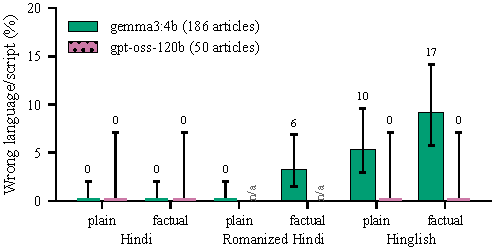
\includegraphics[width=\columnwidth]{fig_wrong_language}
  \caption{Share of summaries in the wrong language or script (95\% Wilson intervals; numbers above bars are counts). gpt-oss-120b was run on 50 articles for \cond{hi} and \cond{hinglish} only.}
  \label{fig:wronglang}
\end{figure}

\begin{figure}[t]
  \centering
  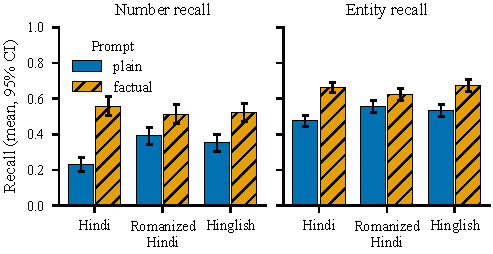
\includegraphics[width=\columnwidth]{fig_recall_by_condition}
  \caption{Number and entity recall of gemma3:4b summaries by condition and prompt (mean with 95\% bootstrap CI; summaries in the wrong language excluded).}
  \label{fig:recall}
\end{figure}

\begin{table*}[t]
\centering
\caption{gemma3:4b, all 186 articles: means over summaries that passed the language check ($n$). P/R = precision/recall. 95\% bootstrap CIs are in \texttt{results/summary\_table\_gemma3\_4b.csv}. NLI is comparable only within a condition.}
\label{tab:main}
\setlength{\tabcolsep}{4.5pt}
\begin{tabular}{@{}llrcccccccccc@{}}
\toprule
Condition & Prompt & $n$ & Num P & Num R & Ent P & Ent R & NLI chunk & NLI window & ROUGE-2 & BERTScore & Words \\
\midrule
\multirow{2}{*}{\cond{hi}}       & plain   & 186 & 0.979 & 0.230 & 0.974 & 0.475 & 0.742 & 0.745 & 0.141 & 0.749 & 73.9 \\
                                 & factual & 186 & 0.970 & 0.556 & 0.994 & 0.661 & 0.613 & 0.727 & 0.259 & 0.787 & 78.6 \\
\multirow{2}{*}{\cond{hi-rom}}   & plain   & 186 & 0.999 & 0.390 & 0.995 & 0.553 & 0.475 & 0.713 & 0.388 & 0.788 & 80.9 \\
                                 & factual & 180 & 1.000 & 0.513 & 1.000 & 0.624 & 0.454 & 0.708 & 0.440 & 0.792 & 84.7 \\
\multirow{2}{*}{\cond{hinglish}} & plain   & 176 & 0.981 & 0.352 & 0.979 & 0.534 & 0.511 & 0.632 & 0.248 & 0.746 & 83.3 \\
                                 & factual & 169 & 1.000 & 0.523 & 0.997 & 0.675 & 0.397 & 0.647 & 0.419 & 0.786 & 87.5 \\
\bottomrule
\end{tabular}
\end{table*}

\begin{table*}[t]
\centering
\caption{gpt-oss-120b vs.\ gemma3:4b on the same 50 articles. Wrong-language rate over all 50 summaries per cell; all other columns are means over the $n$ rows where both models answered in the right language.}
\label{tab:models}
\setlength{\tabcolsep}{4pt}
\begin{tabular}{@{}lllrrcccccccc@{}}
\toprule
Condition & Prompt & Model & Wrong lang. & $n$ & Num P & Num R & Ent P & Ent R & NLI chunk & NLI window & ROUGE-L & Words \\
\midrule
\multirow{4}{*}{\cond{hi}} & \multirow{2}{*}{plain} & gemma3:4b & 0\% & 50 & 0.926 & 0.197 & 0.985 & 0.461 & 0.729 & 0.739 & 0.212 & 75.3 \\
 & & gpt-oss-120b & 0\% & 50 & 0.958 & 0.465 & 0.987 & 0.543 & 0.669 & 0.624 & 0.223 & 76.2 \\
 & \multirow{2}{*}{factual} & gemma3:4b & 0\% & 50 & 0.987 & 0.499 & 1.000 & 0.657 & 0.625 & 0.721 & 0.297 & 78.2 \\
 & & gpt-oss-120b & 0\% & 50 & 0.996 & 0.651 & 0.980 & 0.729 & 0.566 & 0.643 & 0.382 & 96.2 \\
\midrule
\multirow{4}{*}{\cond{hinglish}} & \multirow{2}{*}{plain} & gemma3:4b & 10\% & 45 & 0.994 & 0.311 & 0.962 & 0.590 & 0.576 & 0.623 & 0.312 & 82.7 \\
 & & gpt-oss-120b & 0\% & 45 & 1.000 & 0.457 & 0.987 & 0.605 & 0.510 & 0.545 & 0.309 & 82.8 \\
 & \multirow{2}{*}{factual} & gemma3:4b & 14\% & 43 & 1.000 & 0.504 & 0.996 & 0.675 & 0.445 & 0.642 & 0.428 & 87.0 \\
 & & gpt-oss-120b & 0\% & 43 & 1.000 & 0.660 & 1.000 & 0.742 & 0.422 & 0.569 & 0.429 & 99.1 \\
\bottomrule
\end{tabular}
\end{table*}

\begin{figure}[t]
  \centering
  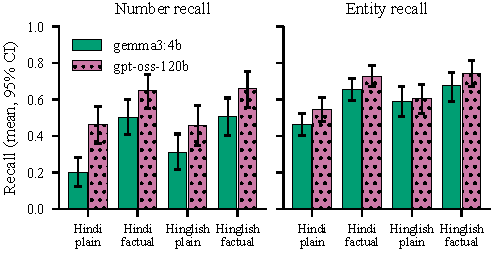
\includegraphics[width=\columnwidth]{fig_model_recall}
  \caption{Number and entity recall of gemma3:4b and gpt-oss-120b on the same 50 articles (188 summaries where both models answered in the right language; 95\% bootstrap CI).}
  \label{fig:models}
\end{figure}

\begin{figure}[t]
  \centering
  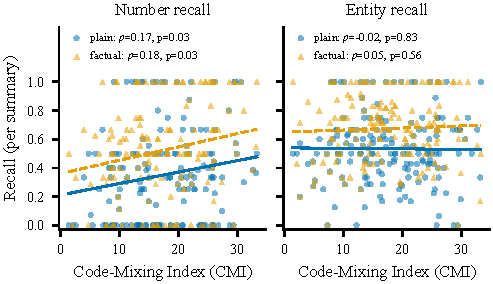
\includegraphics[width=\columnwidth]{fig_cmi_recall}
  \caption{Per-summary recall vs.\ Code-Mixing Index of the source, \cond{hinglish} condition, gemma3:4b, with least-squares lines and Spearman $\rho$.}
  \label{fig:cmi}
\end{figure}

\begin{figure}[t]
  \centering
  \fbox{\parbox[c][3.5cm][c]{0.9\columnwidth}{\centering
    \todo{Figure: agreement of each automatic metric with human labels\\(AUC, faithful vs.\ error, 95\% CI).\\Generated by \texttt{src.analysis.make\_figures} once\\\texttt{src.eval.merge\_annotations} has run.}}}
  \caption{\todo{Metric--human agreement.}}
  \label{fig:agreement}
\end{figure}
